\documentclass[11pt]{beamer}
\usepackage[utf8]{inputenc}
\usepackage[T1]{fontenc}
\usepackage{lmodern}
\usetheme{default}
\usepackage[backend=biber]{biblatex}

\addbibresource{mif_article.bib}
\begin{document}
	\author{Michele De Vita}
	\title{Find Minimal, Maximal and all solutions of Feedback Vertex set}
	%\subtitle{}
	%\logo{}
	%\institute{}
	%\date{}
	%\subject{}
	%\setbeamercovered{transparent}
	%\setbeamertemplate{navigation symbols}{}
	\begin{frame}[plain]
		\maketitle
	\end{frame}
	\begin{frame}{Definition of Feedback Vertex Set}
		Quoting Wikipedia:
		\begin{center}
			\textit{Feedback Vertex Set (FVS) of a graph is a set of vertices whose removal leaves a graph without cycles}
		\end{center}
		
		\small \begin{center} Some examples: \end{center}
		
		\begin{figure}
			\centering
			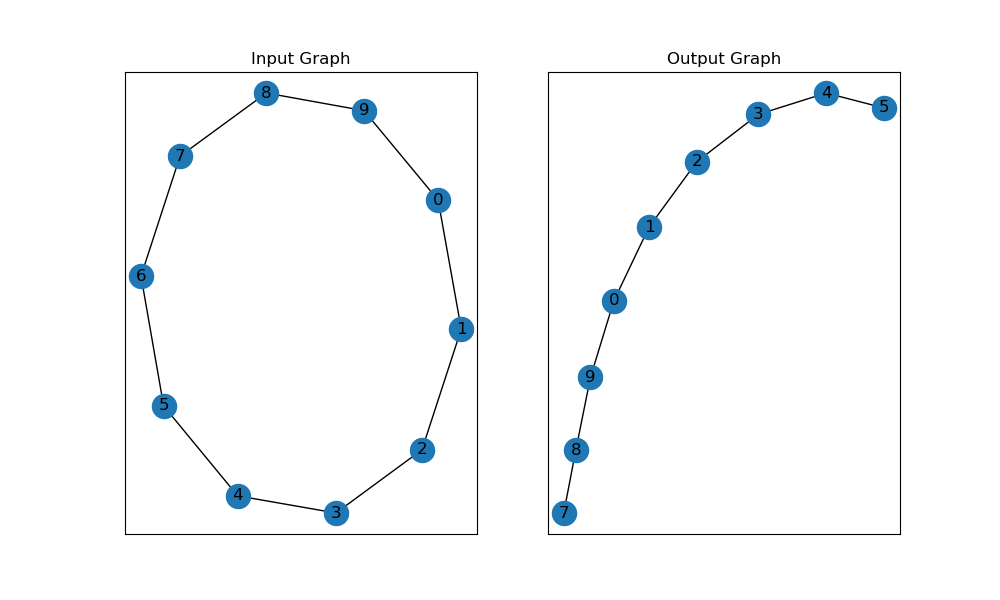
\includegraphics[width=0.45\linewidth]{../plots/cycle_graph}
			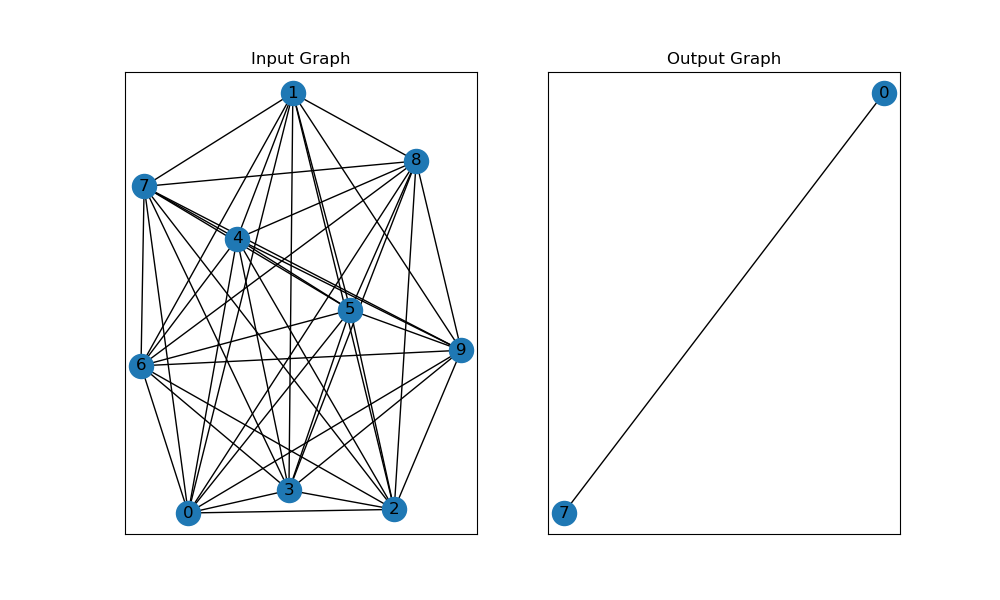
\includegraphics[width=0.45\linewidth]{../plots/complete_graph}
			\label{fig:cyclegraph}
		\end{figure}
		
	\end{frame}
	\begin{frame}{Index}
		\begin{enumerate}
			\item Maximal Feedback Vertex Set
			\item Minimal Feedback Vertex Set
			\item Find all the solution of the Feedback Vertex Set problem
		\end{enumerate}
	\end{frame}
	\begin{frame}{Maximal Feedback Vertex Set}
		\begin{itemize}
			\item A FVS F is maximal if doesn't exists a node x such that $F \cup \left\{ x \right\} $ is a FVS
			\item The solution for Maximal Feedback Vertex Set is trivial with the following propositions:
			\begin{itemize}
				\item Assuming F satisfy FVS property the operation of adding a node to F always satisfy the condition of FVS. In equivalent terms: if G doesn't contain cycles, then remove an additional node from G can't cause any cycle in G 
				\item It always exists a set of nodes $ F \subset V $ that satisfy FVS property: if we take the worst case, a complete graph with n nodes the solution for FVS is all nodes but 2 for any pair of neighbors inside the graph. For all other graphs with n nodes with $ E \subset E_{complete} $ the solution for FVS it's a superset of this.
			\end{itemize}
			\item Therefore the Maximal FVS for graph G is V i.e. the set of all nodes in G.
		\end{itemize}
	\end{frame}
    \begin{frame}{Minimal Feedback Vertex Set}
		\begin{itemize}
			\item The opposite problem is much harder and not trivial to be solved. Furthermore, it has many interesting applications, for instance deadlock solver in a concurrent environment like an OS or DB, chip design and so on.
			\item The complexity of this problem is NP-hard therefore it can be solved in exponential time $O(2^n)$ using a brute force approach, where $ n $ is the number of nodes in G
			\item In this project Minimal FVS is found through a SOTA algorithm \cite{formin} which have time complexity $ O(1.7548^n) $ by solving the dual problem called Maximum Inducted Forest. It consists into finding $ X \subseteq V $ such that $ G\left[ X \right] $ doesn't have cycles and X is maximal. 
			\item This algorithm can be applied only to undirected graphs, so from now on we assume that G is undirected
		\end{itemize}
    \end{frame}
	\begin{frame}{Algorithm for Maximum Inducted Forest}
		\begin{itemize}
			\item The algorithm \textit{find\_mif} consists in a sequence of 11 rules where the i-th rule is applied iff all the previous rules are false. The objective of these rules is either return a solution or to branch the problem in sub-problems.
			\item The algorithm has two main elements:
				\begin{itemize}
					\item F is the set containing the Maximum Inducted Forest
					\item \textit{t} is the active vertex. During the algorithm a neighbor of \textit{t} it's used to branch in many sub-problems.
				\end{itemize}
			\item For instance, the first rule is: \\ \,\, If G has multiple CC (Connected Components) then return: $$ \bigcup_{cc \in G} find\_mif\left(cc, F \cap cc, t \right) $$
			\item Once the Maximum Inducted Forest is found, just return V - MIF to get Minimal Feedback Vertex Set
		\end{itemize}
	\end{frame}
	\begin{frame}{All solution for FVS}
		\begin{itemize}
			\item The search for all the possible solutions for FVS can be divided in two subproblems:
			\begin{enumerate}
				\item Find all FVS with minimal cardinality
				\item Find strictly not minimal FVS 
			\end{enumerate}
			\item  Prop: If we have 1. then 2. it's trivial because any not minimal FVS can be obtained as $ X = F_{min} \cup Y $ where $ Y \in V / F_{min} $. This follows by the first proposition used to find Maximal Feedback Vertex Set, i.e. if F is a FVS then $ F' = F \cup X $ also satisfy the property for any  $ X \in V / F $
		\end{itemize}
	\end{frame}
	\begin{frame}
		\begin{itemize}
			\item Therefore we have reduced the problem to find all solutions to 1), but how to find all minimal FVS?
			\begin{enumerate}
				\item Run algorithm to find a MIF (see Minimal FVS section)
				\item Get all CC
				\item Run n DFS with $ max\_depth=|MIF| $, one for each node $ n_0 $ with slight modifications:
				\begin{enumerate}
					\item $ ancestors = ancestors \cup \left\{ n_0 \right\} $
					\item \textit{if size(ancestors) = |MIF| then return ancestors}
					\item let $ N = \left\{ n: n \in neighbors(G, n_0) \wedge \, ! \exists (n,v) \in E: \, v \in ancestors \right\} $
					\item if $ N = \emptyset $ then $ N = \left\{ n \right\}  $ : $ n \in V \wedge n \notin ancestors \wedge \, ! has\_cycle(G, ancestors \cup \left\{ n \right\})$
					\item if again $ N = \emptyset $ return solutions by recursive calls
					\item for each $ n \in N $ calls recursively $ find\_mif \left( G, ancestors \cup \left\{ n \right\} \right) $
					
				\end{enumerate}
				\item Return FVS solutions as V - MIF for each MIF got from the previous point
			\end{enumerate}
		\end{itemize}
	\end{frame}
	\begin{frame}
		\begin{itemize}
			\item Demonstration of correctness of DFS (For simplicity assume single CC): Assume for absurd that a path P got from DFS isn't a MIF. Then the cases are 2:
			\begin{itemize}
				\item P contains a cycle: this is impossible because the algorithm have a cycle detection procedure
				\item  P is not Maximal: This is impossible because the algorithm returns only path of length |MIF|
			\end{itemize}
			\item Computation cost of the algorithm: $$ O( \underbrace{1.75 ^ n}_{Find \, first \, MIF} + \underbrace{|V| \cdot |MIF|}_{DFSs} \underbrace{\left( |V| + |E|\right) }_{cycle detection})  \approxeq O(1.75^n + n^2) $$
			 In conclusion, the cost to find all all the solutions is approximately equal to the cost to find initially the cardinality of MIF
			 \item This analysis assume that get all supersets of Minimals FVS is $ O(1) $ 
		 	\end{itemize}
	\end{frame}
	\begin{frame}{Bibliography}
		\printbibliography
	\end{frame}
\end{document}